\section{Introduction}
\label{sec:intro:0}

The Vera C. Rubin Observatory's Data Preview 2 (DP2) represents a
significant step forward in preparation for the upcoming Legacy Survey
of Space and Time (LSST), providing an essential testbed for
scientific tools and analytical pipelines using precursor imaging
data~\cite{DMTN-095}. A central goal of LSST is estimating photometric
redshifts (photo-𝑧s) for billions of galaxies, supporting
extragalactic astrophysical research and cosmological studies that
depend on reliable redshift measurements and distributions. In support
of this objective, the Rubin project established a strategic plan for
delivering high-quality photo-𝑧s to the research
community~\cite{DMTN-049}.  

While photo-𝑧 estimates are not part of the official Data Preview 1
(DP1) or DP2 data products, the "Photo-z Science Unit" undertook the
task of producing photo-𝑧 values for all galaxies in DP2 using
available multi-band imaging data on a best-effort basis, establishing
a foundation for future large-scale implementations.   This science
unit delivered redshifts for DP1\cite{Charles2025sitcomtn154, dp1_paper}.

For this purpose, we utilized the RAIL (Redshift Assessment
Infrastructure Layers) software framework, a versatile and modular
tool developed for photo-𝑧 estimation and
validation~\cite{RAIL}. In particular, we leveraged RAIL to
train photo-𝑧 estimation models using high-quality spectroscopic
redshift training samples matched to the DP2 photometric catalog.

This document presents the resulting best-effort photo-𝑧 catalogs,
which should be considered highly preliminary, along with the
methodologies and procedures employed to create them. Furthermore, we
discuss key characteristics of the DP2 photometric data, the
spectroscopic calibration samples, and the resulting photo-𝑧
catalogs. Supplementary information regarding data products and
distribution is provided in the appendices.

We anticipate receiving input from scientific users as they examine
the data and identify issues we may have overlooked, and we plan to
integrate this feedback into subsequent efforts.



\section{Data}
\label{sec:data:0}

\subsection{Rubin DP2}
\label{sec:data:dp1}

The Rubin Observatory’s Data Preview 2 dataset is the first public release of Rubin observatory imaging data from the full LSST camera processed through the LSST Science Pipelines~\citep{PSTN-019}, serving as a critical testbed for scientific and technical validation ahead of full LSST operations.  DP2 is based on observations from the LSST camera (LSSTCam) and includes multi-band optical imaging in u, g, r, i, z and y filters over $>$ 1000 square degrees of sky.  The dataset consists of processed images, source catalogs, and associated metadata, all formatted using the Rubin Data Butler system~\citep{2022SPIE12189E..11J}.  Although somewhat smaller in scale than future LSST datasets, DP2 offers realistic photometric measurements, object detection, and data structures, making it an invaluable resource for developing and testing algorithms for tasks such as \photoz estimation, object classification, and data quality assessment.

Critically, the fields selected for commisioning observation included several calibration fields, for which many high-quality redshifts exist from other surveys. 


\subsubsection{Preparation of photometric object catalogs}
\label{sec:data:dp1:preparation}

The Rubin Data Management (Rubin DM) pipeline measures multiple types of object photometry, the first stage in creating a \photoz catalog was to determine which measured photometry we would use as inputs.  In this note, we generally use the 1.0 arc-second Gaussian Aperture fluxes and their associated errors, e.~g.~\texttt{u\_gaap1p0Flux} and \texttt{u\_gaap1p0FluxErr}.  These fluxes should provide good measures of consistent galaxy colors within the defined aperture, ideal for \photoz estimation, though they may not necessarily reflect the colors of the overall galaxy if there is a significant color gradient and the galaxy is larger than the 1.0 arc-second aperture.  This choice of photometric measurement may not be ideal, and investigation into the optimized set of photometric inputs will continue into the future.   This is similar to studies done with DP1 and described in the associated technote and paper~\cite{Charles2025sitcomtn154, dp1_pz_paper}.

Preparing object catalog~\citep{RubinObs2025DP1} data for \photoz algorithm training and estimation included five steps:

\begin{enumerate}
\item{Applying quality cuts to the object catalog.   We developed selections for the training and test datasets (\selection{match\_xxx}), and two additional selections for full DP1 catalogs: one applicable for fields with observations in only four bands (\selection{gold\_4\_band}), the other for fields with observations in all six bands (\selection{gold}).  These selections are described below.}
\item{Converting fluxes in nJy to AB magnitudes ($m_{\rm AB} = -2.5 \log_{10}(f_\nu / \text{nJy}) + 31.4$)}
\item{De-reddening to account for Galactic dust.  We use the SFD dust maps\citep{SFD}.}
\item{Cross-matching objects with reference catalogs that include redshift information as described in Sec.~\ref{sec:data:reference}.}
\item{Shuffling and splitting the resulting catalog into \dataset{training} and \dataset{test} data sets.}
\end{enumerate}

\subsubsection{Data properties}


We have developed tools to generate diagnostic plots of both the input object catalogs and the \photoz estimates as part of our data analysis.
Fig.~\ref{fig:dp_mags} shows histograms of the AB magnitudes in 1.0 arc-second apertures of objects in the \dataset{test\_v1} dataset, which includes an explicit magnitude cut, $m_{i} < 26.0$.
Fig.~\ref{fig:dp_mag_i_v_redshift} shows the correlation between magnitude and redshift for all objects in the \dataset{test\_v1} data set.  
Fig.~\ref{fig:dp_color_v_redshift} shows the ``adjacent band colors'', i.e., $u-g$, $g-r$, $r-i$, $i-z$, $z-y$ versus redshift for the same, with a series of SED templates (as used by template-fitting algorithms, see Sec.~\ref{sec:method:template}) overlaid.  
Finally, Fig.~\ref{fig:dp_color_v_color} shows the color-color plots for the same adjacent colors.  In all cases, the 1.0 arc-second aperture magnitudes are used for plotting.

\begin{figure*}
    \centering
    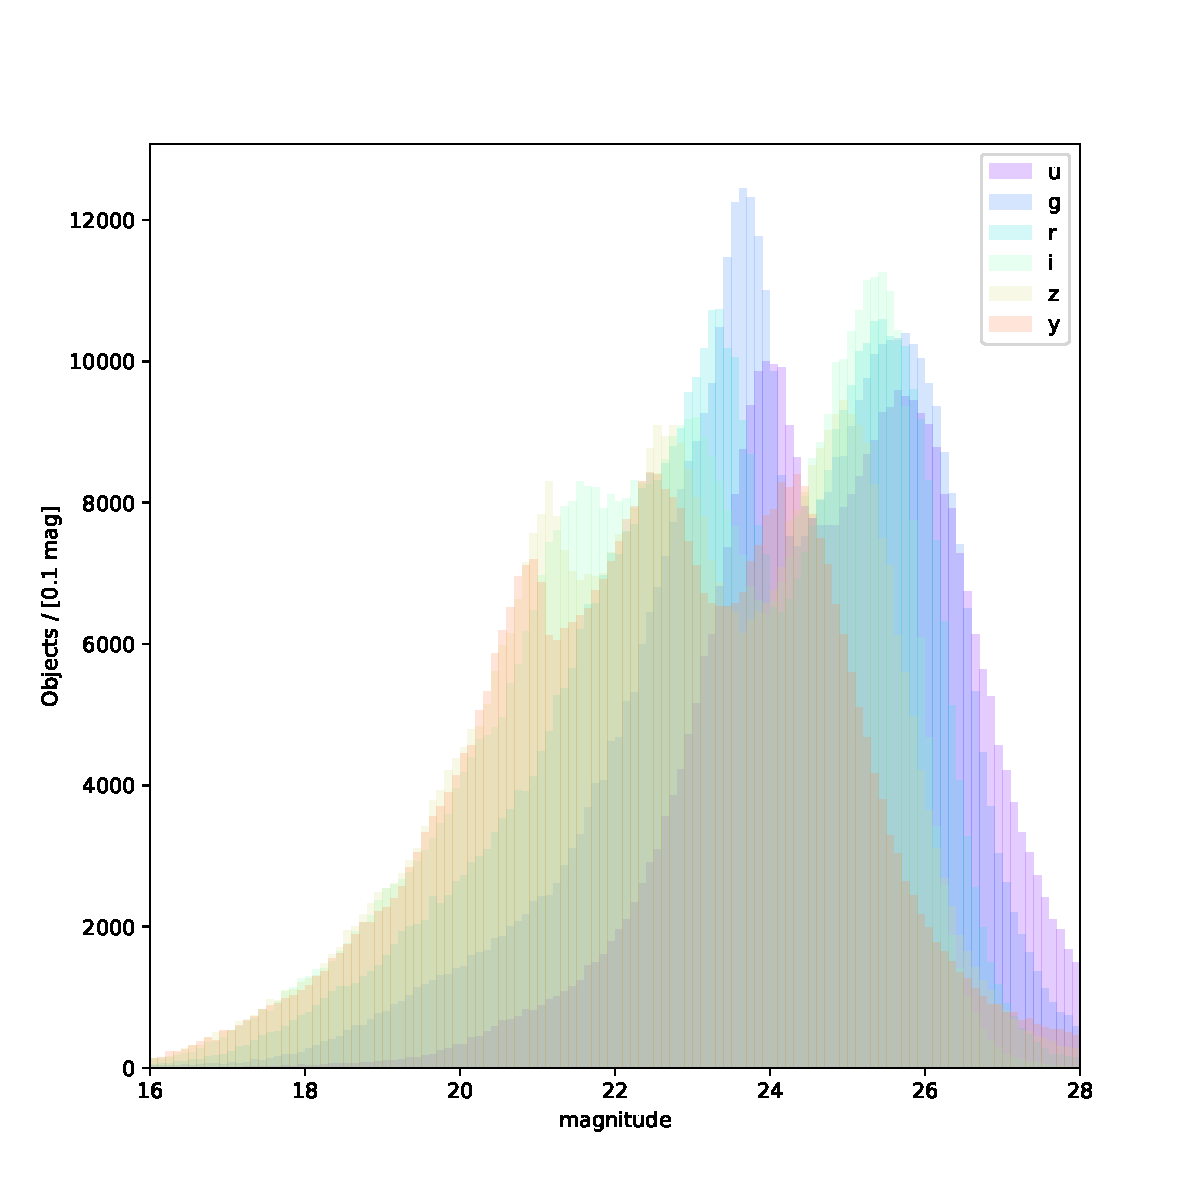
\includegraphics[width=\linewidth]{figures/mags.pdf}
    \caption{1.0 arc-second Gaussian Aperture (Gaap) magnitudes (in AB system) of objects in each of the six Rubin filter bands in the \dataset{test\_v1} dataset.  These aperture magnitudes were used as the inputs for the \photoz algorithms.}
    \label{fig:dp_mags}
\end{figure*}

\begin{figure*}
    \centering
    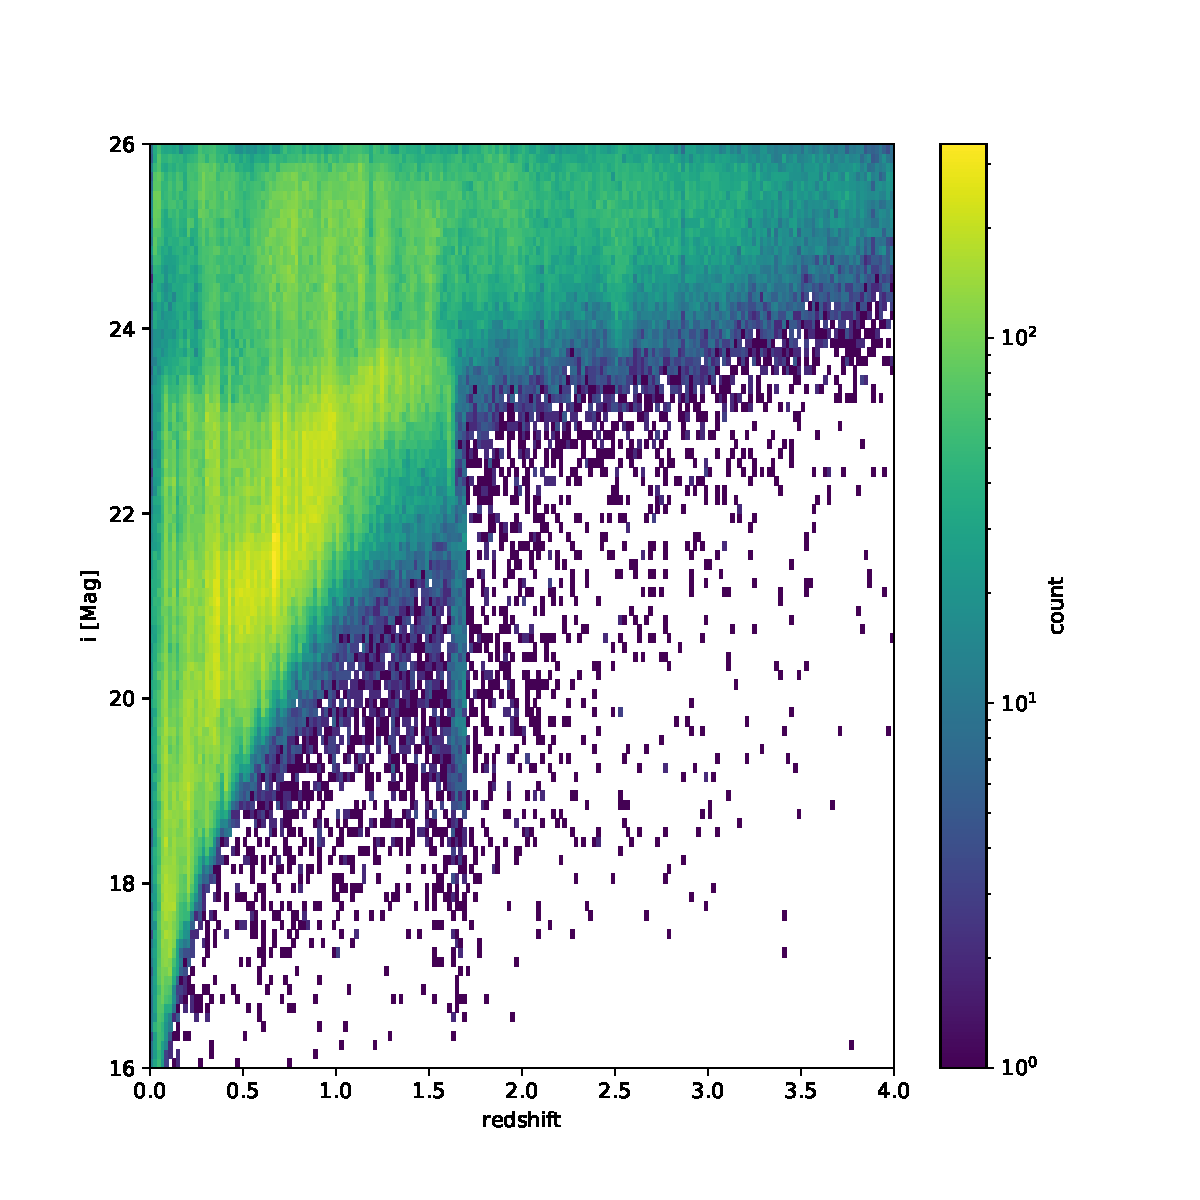
\includegraphics[width=\linewidth]{figures/mag_i_v_redshift.pdf}
    \caption{1.0 arc-second Gaussian Aperture (Gaap) i-band magnitude versus redshift for all objects in the \dataset{test\_v1} dataset.}
    \label{fig:dp_mag_i_v_redshift}
\end{figure*}

\begin{figure*}
    \centering
    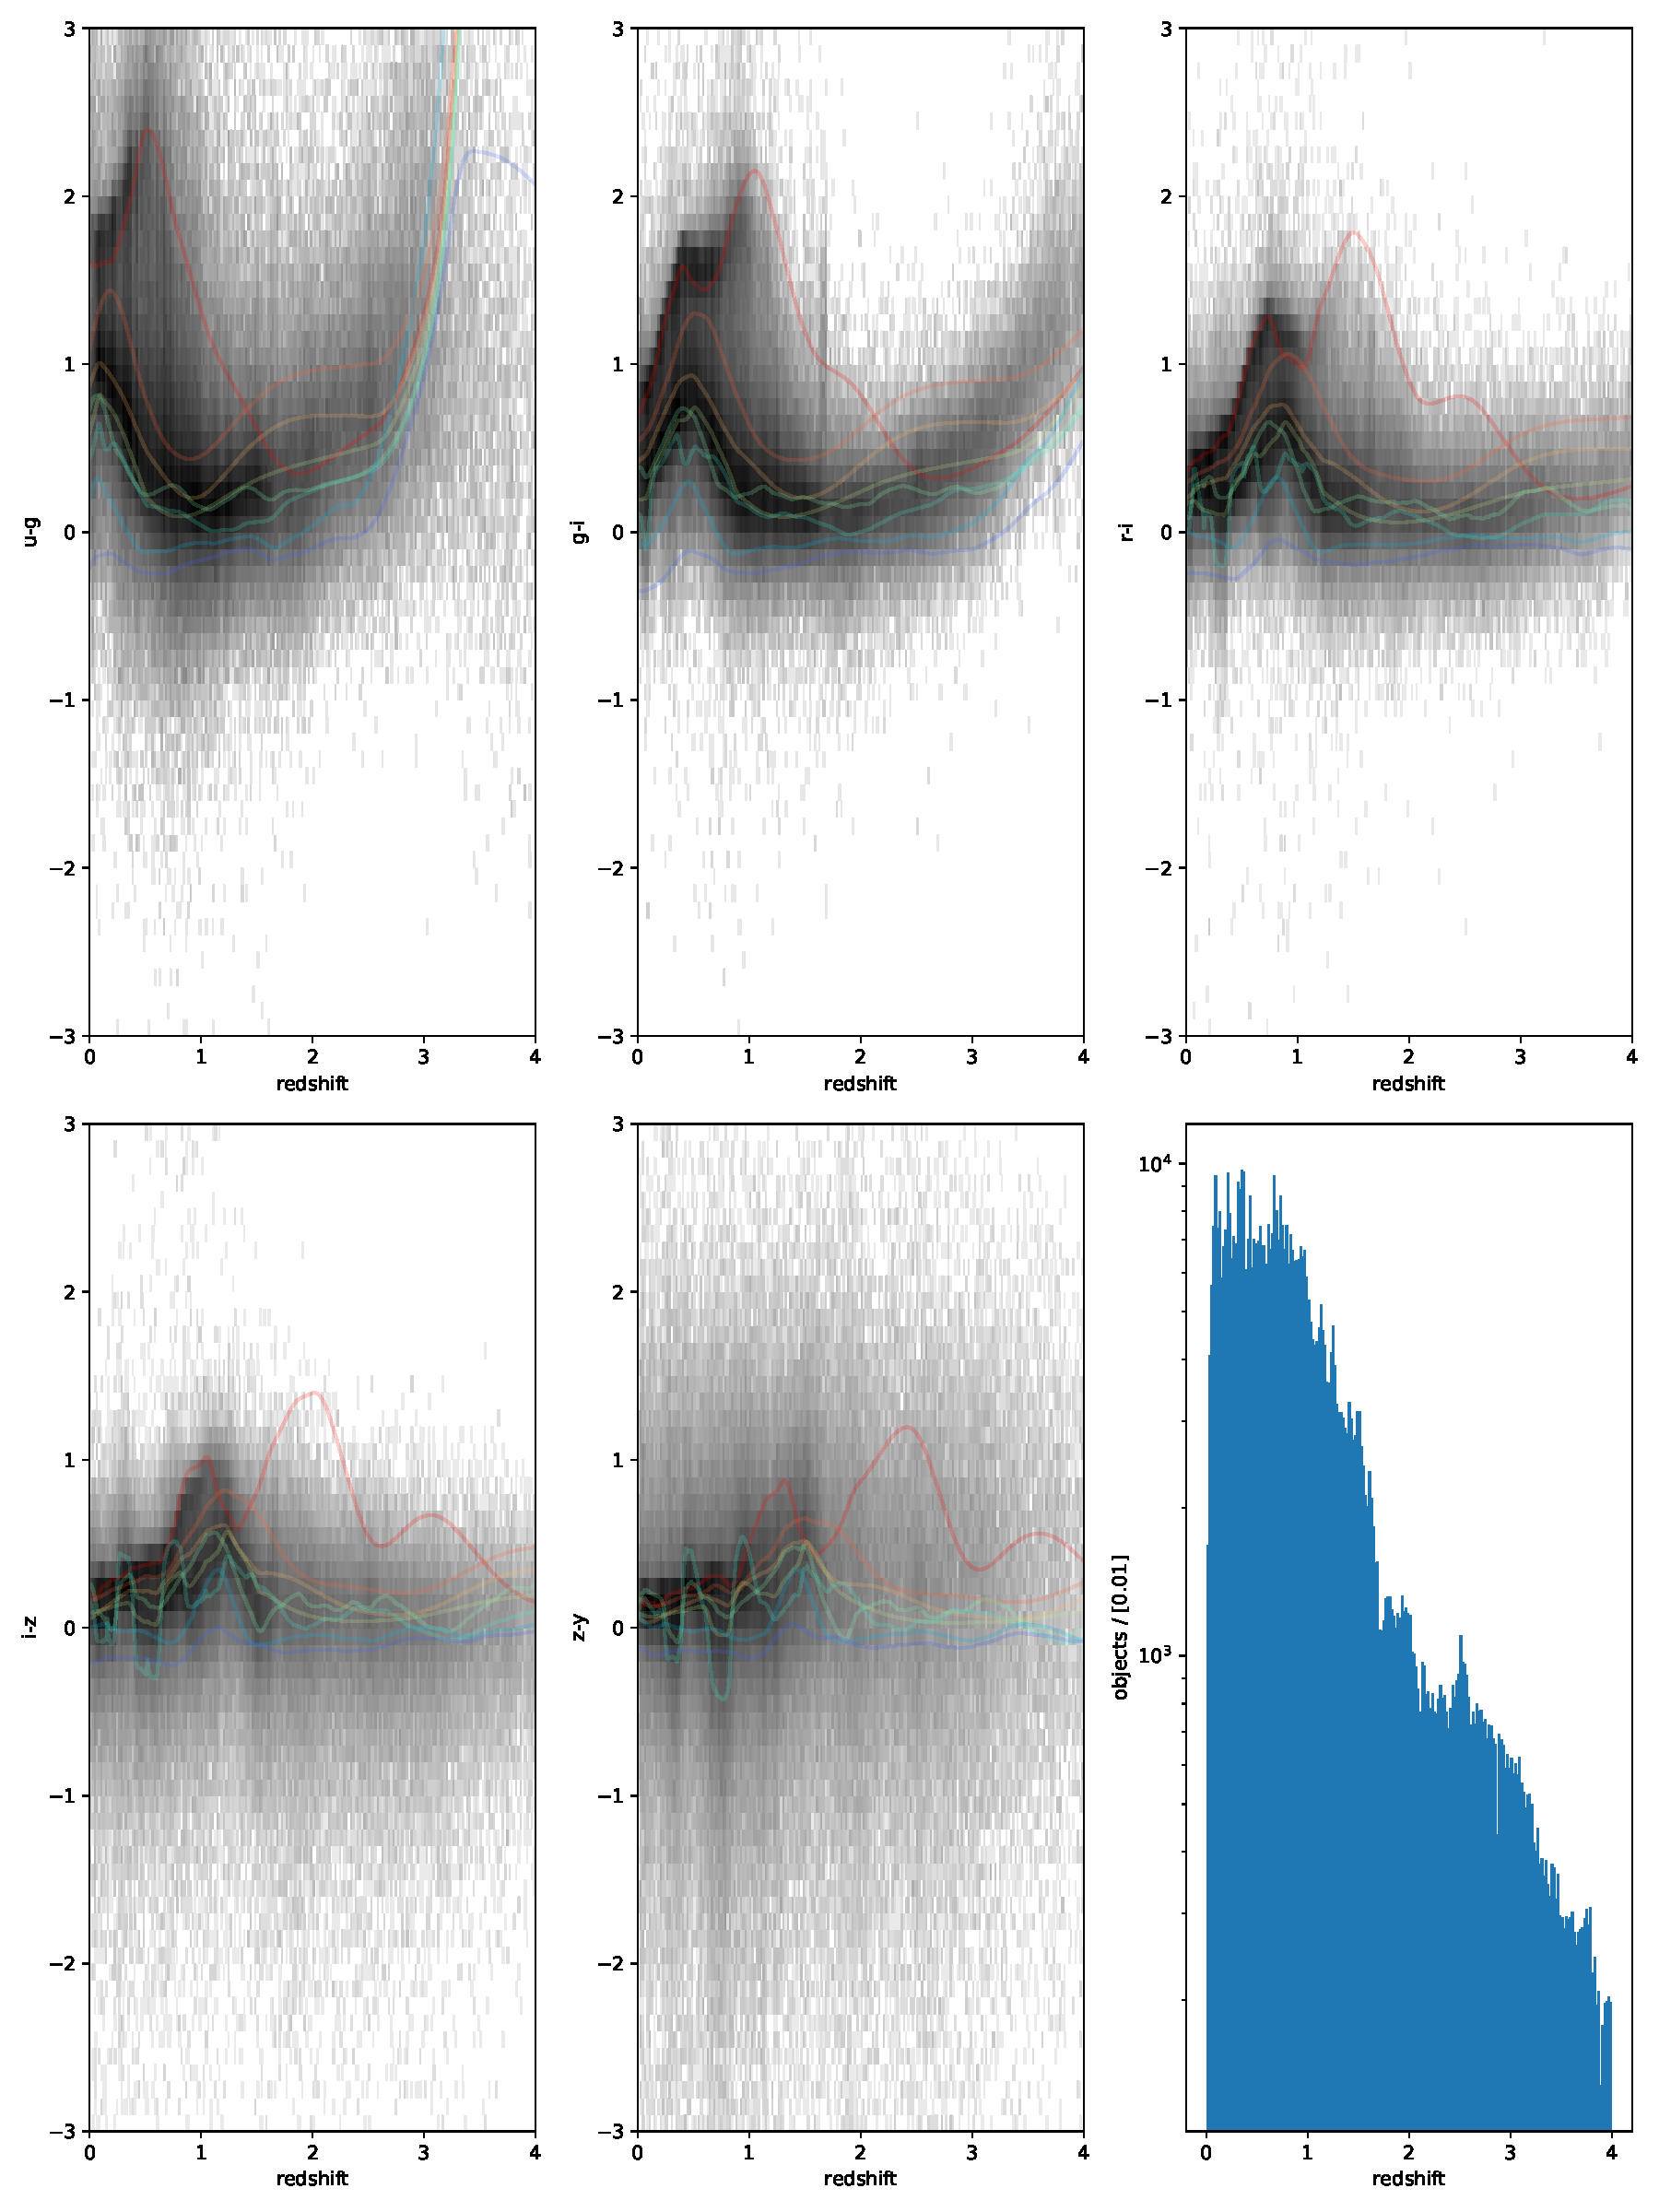
\includegraphics[height=7in]{figures/color_v_redshift.pdf}
    \caption{``Adjacent band colors'', i.e., $u-g$, $g-r$, $r-i$, $i-z$, $z-y$, in 1.0 arc-second apertures versus redshift for all objects in the \dataset{test\_v1} dataset.  Colored lines represent the expected colors for the eight ``CWWSB'' SEDs described in Sec.~\ref{sec:method:template}, and should very roughly show the predicted range of color evolution expected for our galaxy sample.}
    \label{fig:dp_color_v_redshift}
\end{figure*}

\begin{figure*}
    \centering
    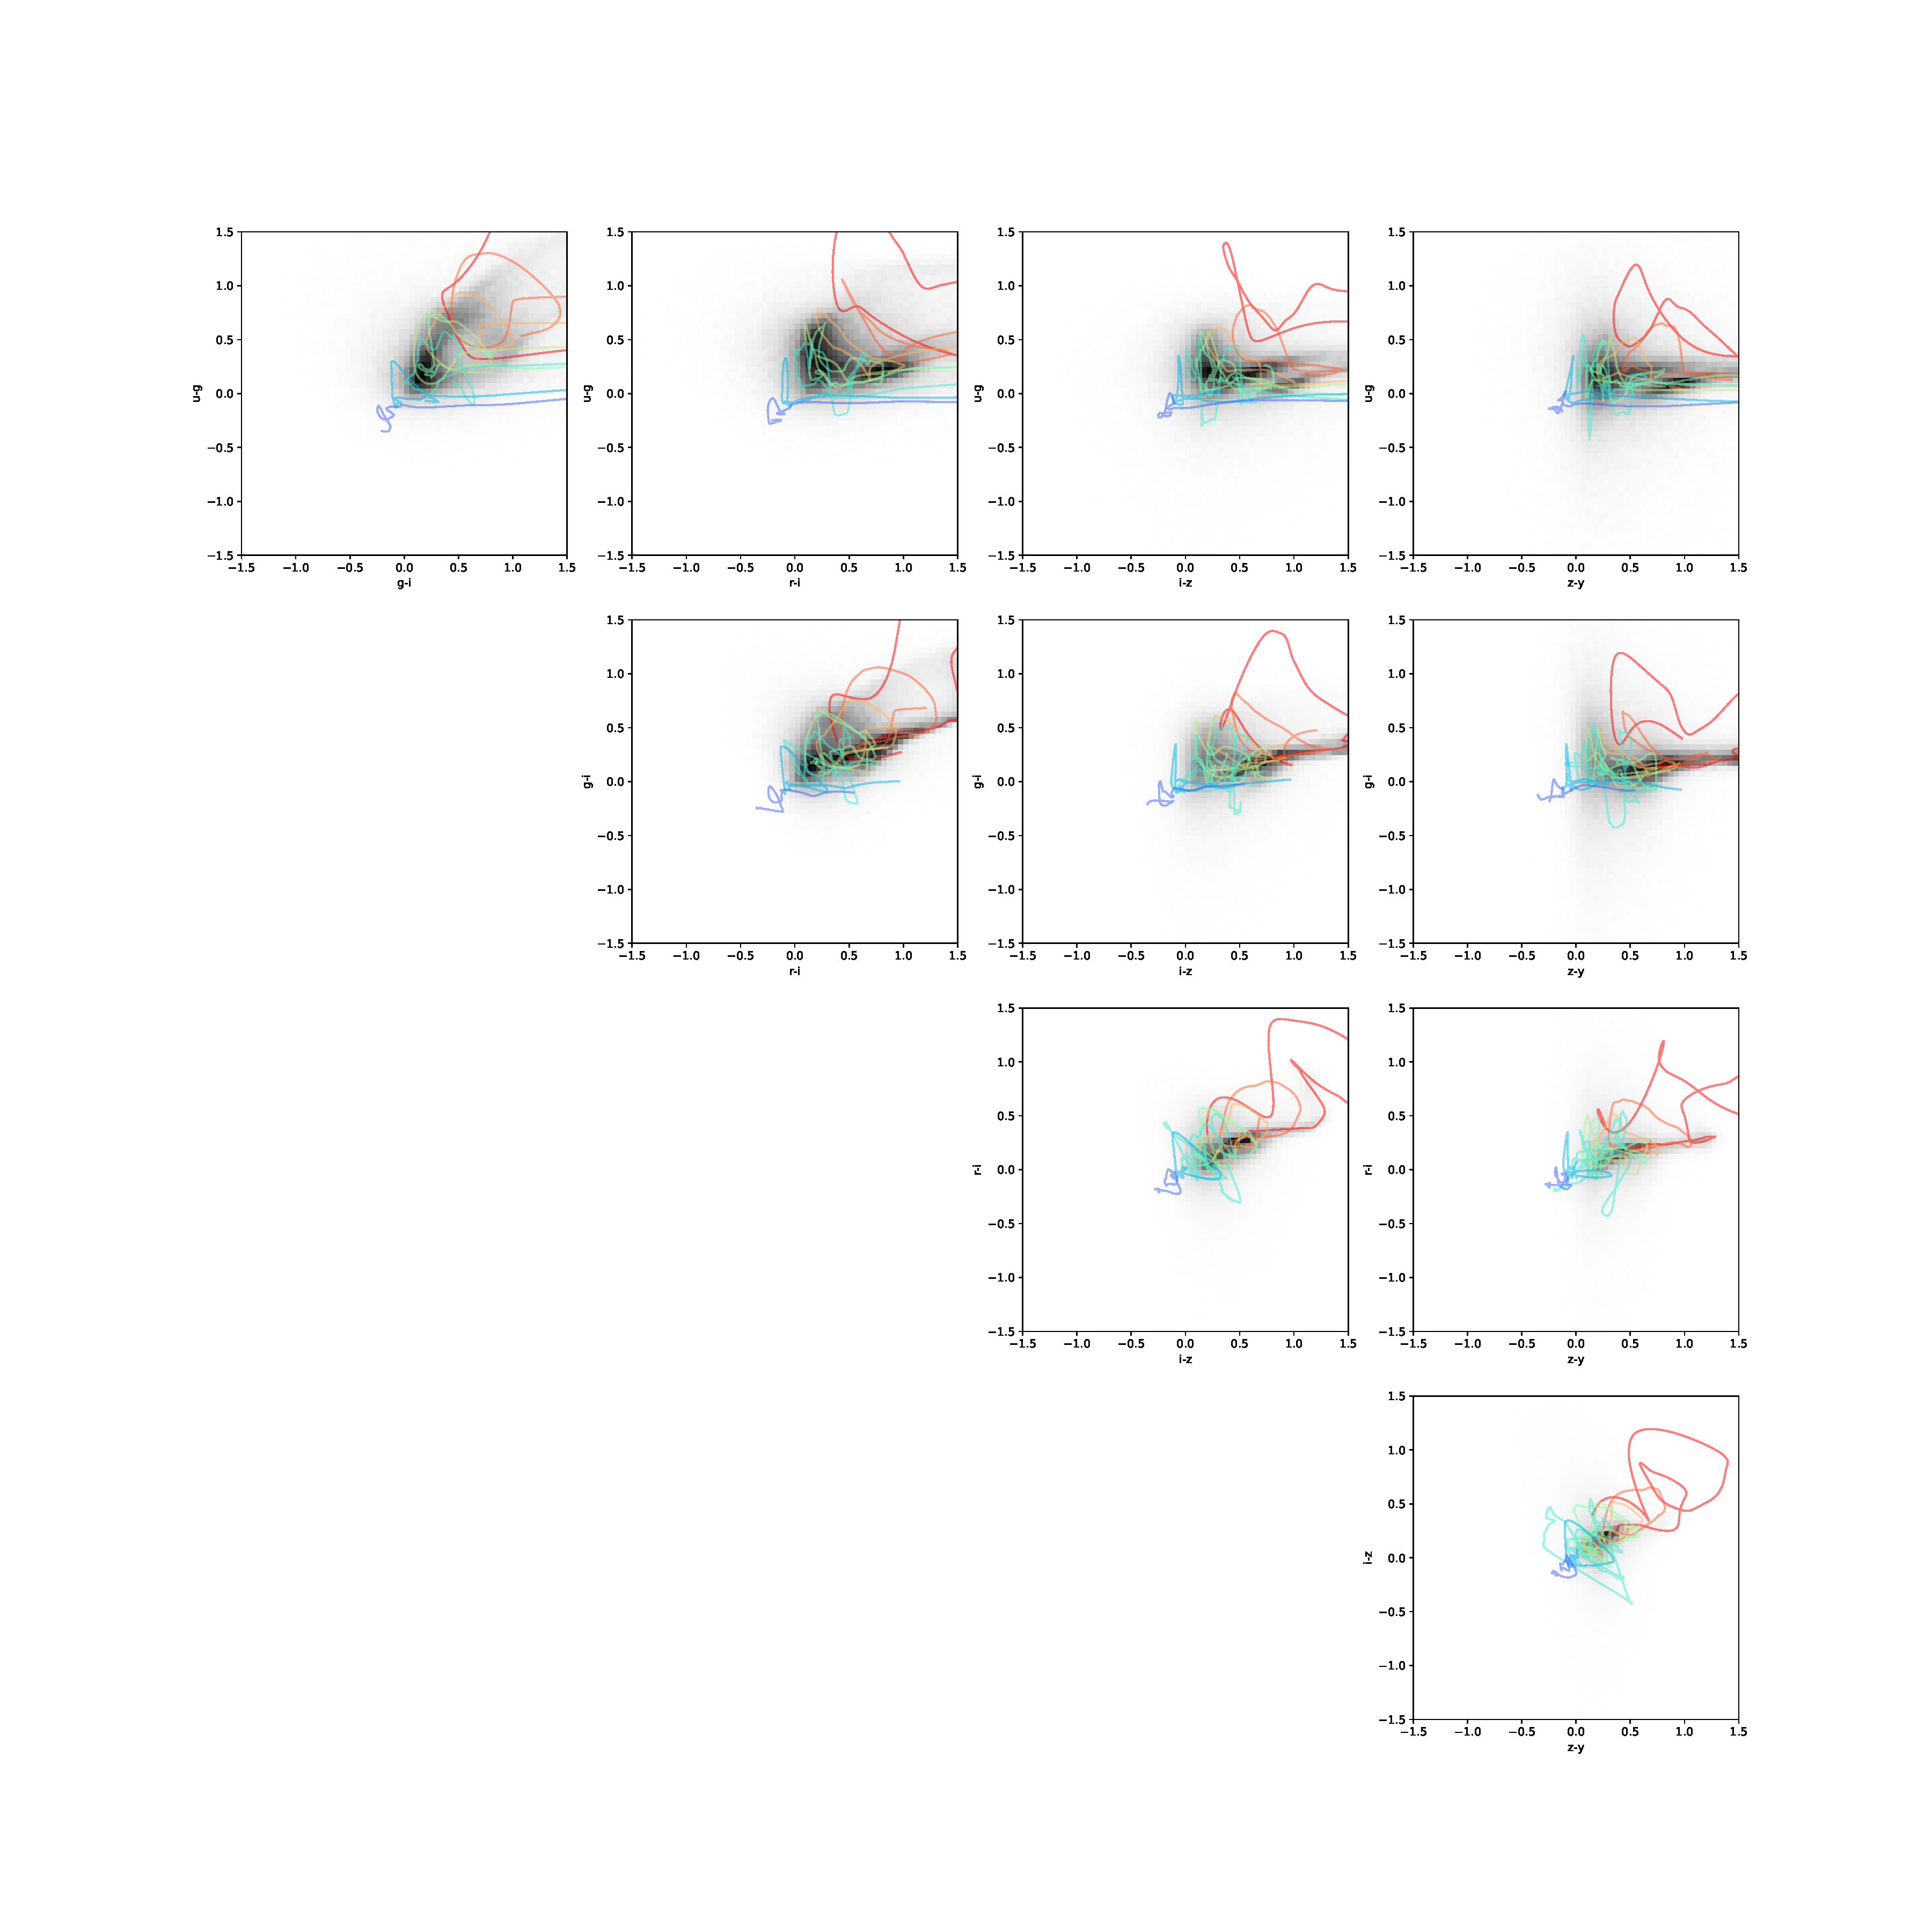
\includegraphics[width=\linewidth]{figures/color_v_color.pdf}
    \caption{Color-color plots for all objects in the `\dataset{test\_v1} dataset.  Colored lines represent the expected colors for the eight ``CWWSB'' SEDs described in Sec.~\ref{sec:method:template}, and should very roughly show the predicted color evolution expected for our galaxy sample.}
    \label{fig:dp_color_v_color}
\end{figure*}


\subsection{Redshift reference sample}
\label{sec:data:reference}

The \photoz estimation algorithms in RAIL require highly accurate and precise redshift estimates cross-matched to the DP1 photometric catalog to provide labeled \dataset{training} data sets.  We created such datasets using data drawn from publicly available catalogs, comprising galaxies with known spectroscopic redshifts, grism redshifts, and high-quality \photoz's from deep multi-band imaging.  These training sets enable machine learning models within RAIL to learn the mapping between galaxy colors and redshifts, enabling \photoz estimation for every galaxy detected in DP1.

TQ...

\section{Methodology}

We used the RAIL as the core tool for training and applying \photoz estimation models.   We also used RAIL to evaluate the model performance through a suite of diagnostic metrics using \photoz point estimates, including redshift bias, scatter (e.g., normalized median absolute deviation), and catastrophic outlier rate and to make diagnostic plots of the algorithm's performance.  Specifically, we used the methodology described below to evaluate all the algorithms listed in Tab.~\ref{tab:alg}.

As part of the Rubin \photoz roadmap process, \code{KNN} and \code{BPZ} were chosen as ``testing algorithms'' from the shortlist of algorithms considered in~\citep{DMTN-049}, the expectation is that these will supported by project data management team for Data Preview 2,  while the others will be supported by the wider community, the RAIL development team and DESC collaboration.

\begin{table*}[ht]
\centering
\begin{tabular}{lll}
 \hline
    Algorithm name  & Home package & Reference\\
 \hline
 \hline
 \multicolumn{3}{c}{Project Supported Testing} \\ 
  \code{BPZ} & \href{https://github.com/LSSTDESC/rail_bpz}{\code{rail-bpz}} & \citet{Benitez:2000}\\
 \code{KNN} & \href{https://github.com/LSSTDESC/rail_sklearn}{\code{rail-sklearn}} & \citet{RAIL} \\
 \multicolumn{3}{c}{Community Supported} \\   
 \code{DNF} & \href{https://github.com/LSSTDESC/rail_dnf}{\code{rail-dnf}} & \citet{2016MNRAS.459.3078D}\\
 \code{FlexZBoost}  & \href{https://github.com/LSSTDESC/rail_flexzboost}{\code{rail-flexzboost}} & \citet{Izbicki:2017}\\
 \code{GPz} & \href{https://github.com/LSSTDESC/rail_gpz_v1}{\code{rail-gpz-v1}} & \citet{Almosallam:2016}\\
 \code{LePHARE} & \href{https://github.com/LSSTDESC/rail_lephare}{\code{rail-lephare}} & \citet{1999MNRAS.310..540A}\\
 \code{TPZ} & \href{https://github.com/LSSTDESC/rail_tpz}{\code{rail-tpz}} & \citet{Carrasco-Kind:2013}\\
 \hline
\end{tabular}
\caption{
Summary of the pre-wrapped estimators/summarizers/classifiers used in this paper and described detail in~\citep{RAIL}.}
\label{tab:alg}
\end{table*}



\subsection{Template fitting based estimators}
\label{sec:method:template}

RAIL’s template-based fitting algorithms (\code{Lephare} and \code{BPZ}, see references in Tab.~\ref{tab:alg} for more details) estimate photometric redshifts by comparing observed galaxy photometry to a set of predefined theoretical or empirical galaxy templates.  These templates represent a range of galaxy spectral energy distributions (SEDs) that are meant to span the expected range of galaxy types observed in the Universe.  Synthetic model fluxes are computed by red-shifting each SED to a set grid of values and convolving with the Rubin filter curves,  which characterizes the expected variation in observed colors with redshift.  Our algorithms calculate the chi-square/likelihood for each SED at each grid point by comparing the model fluxes in our photometric bands to the observed fluxes and uncertainties.  This process enables the algorithm to determine the relative likelihood for each redshift for a given galaxy by identifying the template that best matches its observed color signature.  An optional empirical Bayesian prior can also be applied to produce a posterior probability rather than a straight likelihood if information on the expected distributions are available.  The training phase for these algorithms consist mostly of preparing pre-computed tables for the expected fluxes in each filter band for each SED template. 

Two sets of templates are included in the \code{rail\_base} software package and used in this note: the ``CWWSB'' templates that are the default templates used by \code{rail\_bpz} and described in \citet[]{Coe:06}, consisting of eight total SEDs, one Elliptical template, two Spiral templates, and five Irregular/Starburst template.  In this note, these SEDs are used to compute synthetic colors that we compare to the observational data in Figures~\ref{fig:dp_color_v_redshift} and~\ref{fig:dp_color_v_color}, but are otherwise not used.  The second template set consists of those described in \citet[]{Ilbert:09}, consisting of 31 synthetic SEDs (including some that are ``interpolated'' between adjacent templates by taking the mean of the two SEDs).  These SEDs are included with \code{rail\_lephare} as ``COSMOS\_mod.list'' in the \code{lephare-data} package.  These SEDs are used by both template codes \code{rail\_bpz} and \code{rail\_lephare}.  The 31 base SEDs contain no internal dust extinction, \code{rail\_lephare} is configured to include dust automatically, while \code{rail\_bpz} required dust to be added explicitly, and additional SED templates that include internal extinction added to the input SED list. \code{LePhare} also includes a set of stellar and AGN SEDs, which are available in the \code{lephare-data} package.


\subsection{Machine learning based estimators}
\label{sec:method:machine_learning}

RAIL’s machine learning algorithms (\code{CMNN}, \code{DNF}, \code{FlexZBoost}, \code{GPZ}, \code{KNN}, \code{TPZ}) are described in detail in the publications listed in Tab.~\ref{tab:alg}.  In short these algorithms attempt to perform a regression analysis to estimate the redshift from the input photometric data.   It is a well-known limitation of machine learning algorithms that they exhibit biases when presented with non-representative data, or are asked to extrapolate results outside region of their training data.


\subsection{Analysis framework and bookkeeping software}
\label{sec:method:rail_project}

The \code{rail\_projects} software package within the RAIL ecosystem provides an essential framework for managing and organizing large-scale photometric redshift estimation workflows.  It acts as a project management and book-keeping tool that helps users streamline their research, especially when working with complex or large datasets, like those associated with the Rubin DP1 data.  The primary focus of \code{rail\_projects} is to offer a systematic way to track different stages of data processing, model training, evaluation, and results across multiple experiments, ensuring that all tasks are well-documented and reproducible.

Additionally, \code{rail\_projects} facilitates the management of large datasets by organizing data into structured directories and providing interfaces for batch processing.  It allows users to scale up their work to handle not only large catalogs of objects but also multiple datasets and redshift estimation tasks.  The package ensures that datasets and models are kept in sync across various stages, from raw input data to intermediate results to final outputs, and makes it easier to systematically export data coherent products.


\subsection{Data exploration and algorithm optimization}
\label{sec:method:optimization}

We explored dozens of different configuration settings, covering analysis choices such as which flux measurements to use, the machine learning hyper-parameters, which sets of SED templates to use, among others.   The \href{https://github.com/LSSTDESC/rail_project_config/blob/main/dp1/dp1.yaml}{dp1/dp1.yaml} configuration file (see Sec.~\ref{sec:products:configuration}) captures the set of configurations that we tested and labels each set into an analysis ``flavor'' to facilitate bookkeeping. 

After examining the performance of the algorithms under different configurations, we settled on a set of optimized parameters for each algorithm and on the \code{gaap\_1p0} fluxes to produce the best-effort catalogs for DP1.   These optimized configurations parameters are captured in the \href{https://github.com/LSSTDESC/rail_project_config/blob/main/dp1/dp1_v4.yaml}{dp1/dp1\_v4.yaml} configuration file.


\subsection{Production of redshfits catalogs}
\label{sec:method:redshift_catalogs}

We also used the \href{https://github.com/lsst-dm/meas_pz}{\code{meas\_pz}} and \href{https://github.com/lsst-dm/meas_pz}{\code{meas\_pz\_extensions}} software packages
to create \photoz catalogs in the Rubin data management framework.

Specifically, we imported trained models produced in the \code{rail\_project} into the DP1 data Butler and produced \photoz estimates for every object in DP1 for each algorithm.

We did this for the \texttt{baseline} analysis flavor, (consisting of ``out-of-the-box'' algorithms, with all settings at default values) and the optimized 6 band (\texttt{dp1\_optimize}) flavor defined in \href{https://github.com/LSSTDESC/rail_project_config/blob/main/dp1/dp1_v1.yaml}{dp1/dp1\_v1.yaml}.
The resulting data products are internally available via data Butlers at USDF and NERSC as described in App.~\ref{sec:distribution:butler}.   As with the \code{rail\_projects} created catalogs, it is expected some of the products will be distributed via other methods in the near future (see App.~\ref{sec:distribution:linea} and App.~\ref{sec:distribution:lsdb}).


\section{Performance}
\label{sec:performance:0}

We evaluated all the algorithms listed in Tab.~\ref{tab:alg} for both scientific and technical performance.


\subsection{Redshift estimator performance}


\subsubsection{Redshift estimation quality flags}
\label{sec:performance:pz:flag}


Applying a simple cut on the RMS of the $p(z)$ distribution can dramatically reduce the catastrophic outlier rate.  In Fig.~\ref{fig:perf_quality_cut} we show how the efficiency and purity obtained on the test sample varies with a single additional cut, $x$ in $\sigma_{p(z)} < x$.   In Fig.~\ref{fig:scatter_quality_cut} we show how applying a cut at $\sigma_{p(z)} < 0.15$ improves the scatter of the photometric redshift point-estimate versus spectroscopic redshift distribution.  As fainter objects and objects at higher redshift often have larger $p(z)$ RMS values, cuts on RMS will likely result in relative shifts in the magnitude and redshift distribution depending on the cut value.

\begin{figure*}
    \centering
    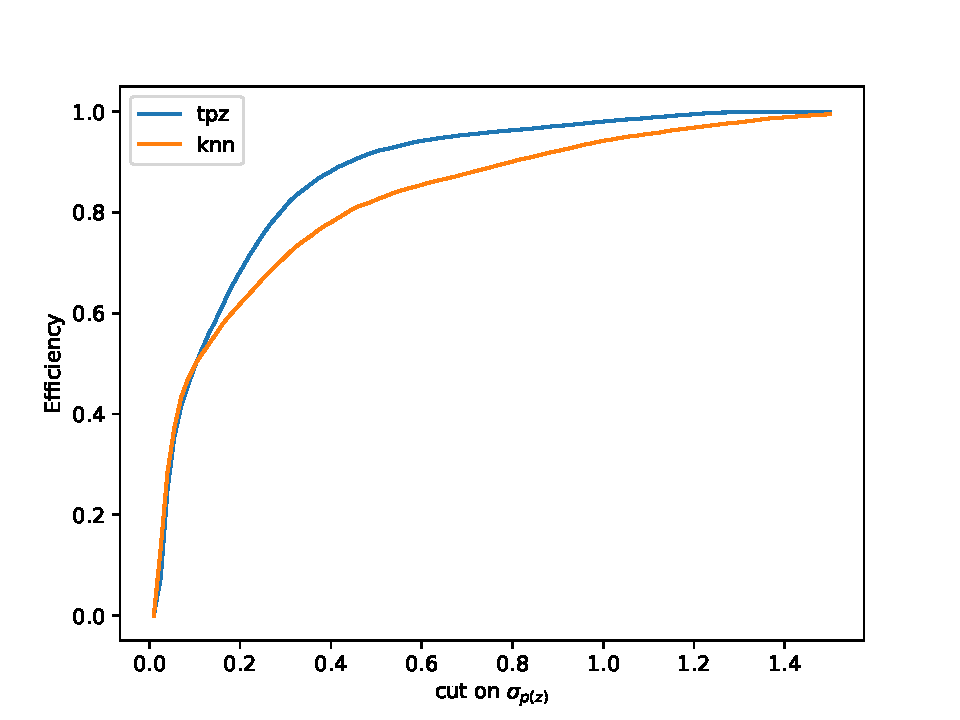
\includegraphics[width=0.45\linewidth]{figures/efficiency.pdf}
    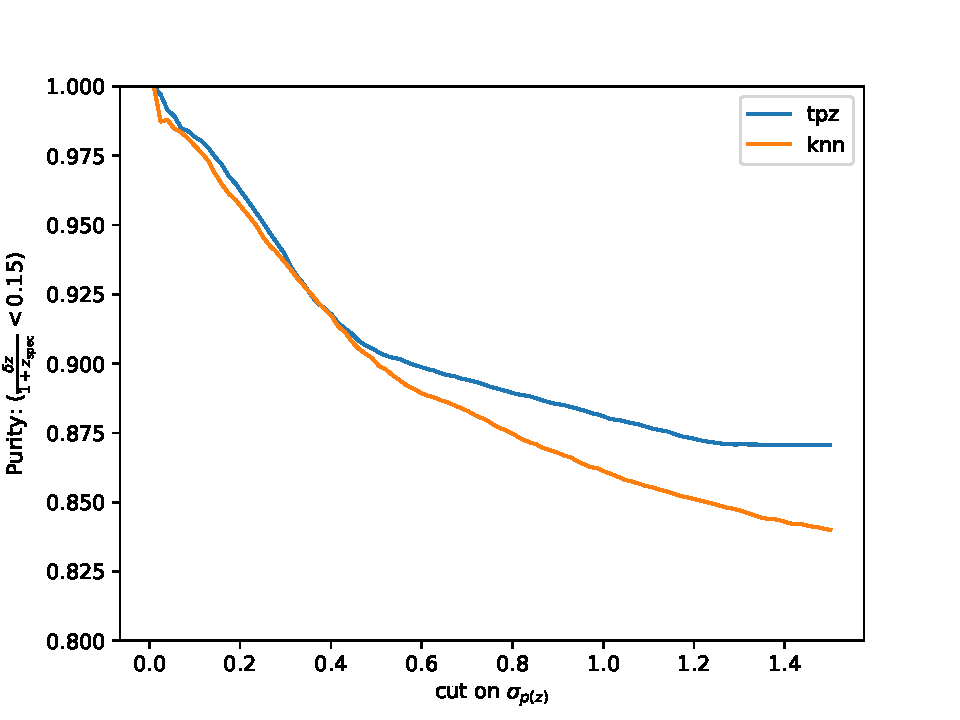
\includegraphics[width=0.45\linewidth]{figures/purity.pdf} \\
    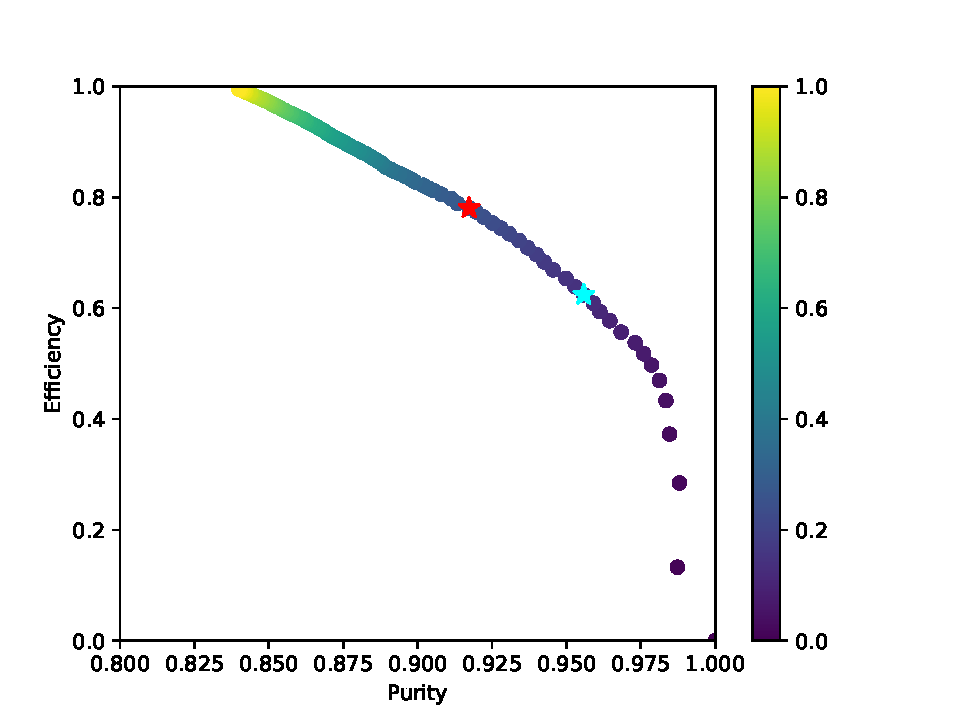
\includegraphics[width=0.45\linewidth]{figures/purity_v_effic.pdf} \\
    \caption{Efficiency (top left) and ``purity'', i.e., fraction of objects with $\frac{\delta z}{1 + z_{\rm spec}} < 0.20$) (top right) versus quality cut, $x$ in $\sigma_{p(z)} < x$.   Bottom, purity version efficiency with cut value shown by the color scale.   The red star shows the point for a cut value  $\sigma_{p(z)} < 0.15$.}
    \label{fig:perf_quality_cut}
\end{figure*}

\begin{figure*}
    \centering
    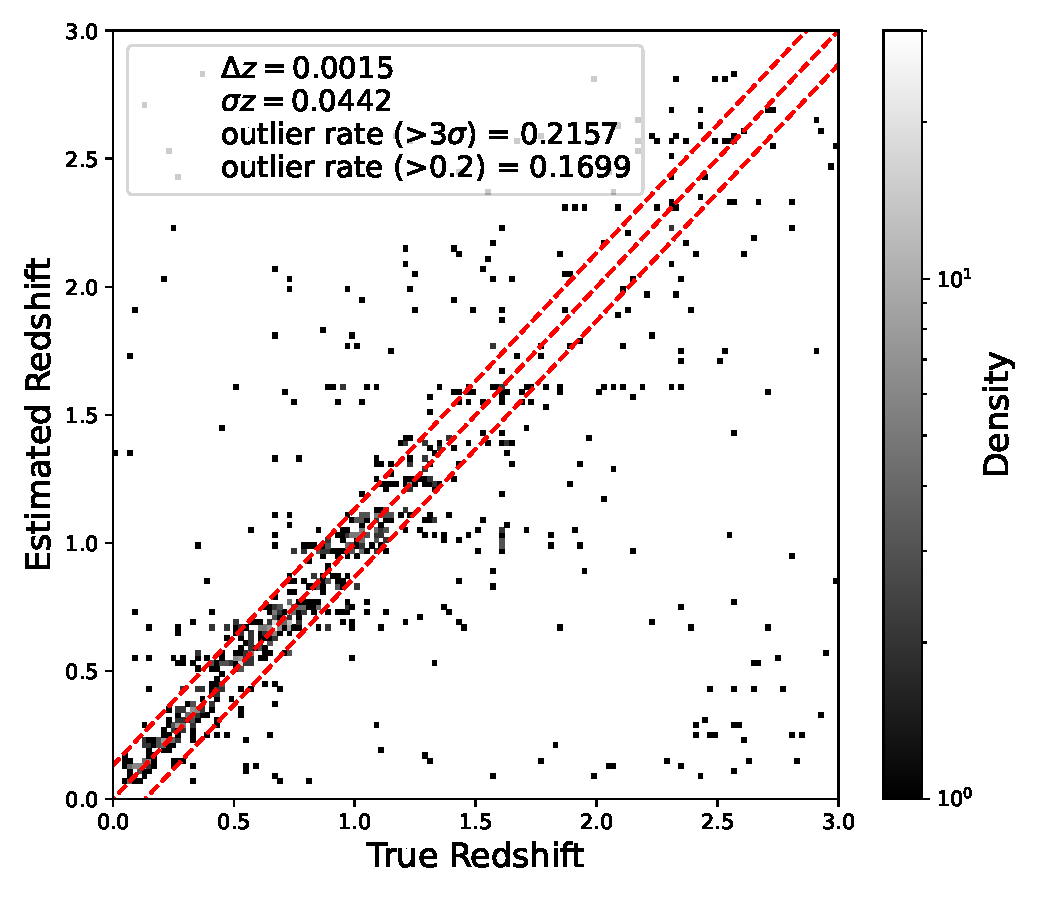
\includegraphics[width=0.45\linewidth]{figures/tpz_scatter_orig.pdf}
    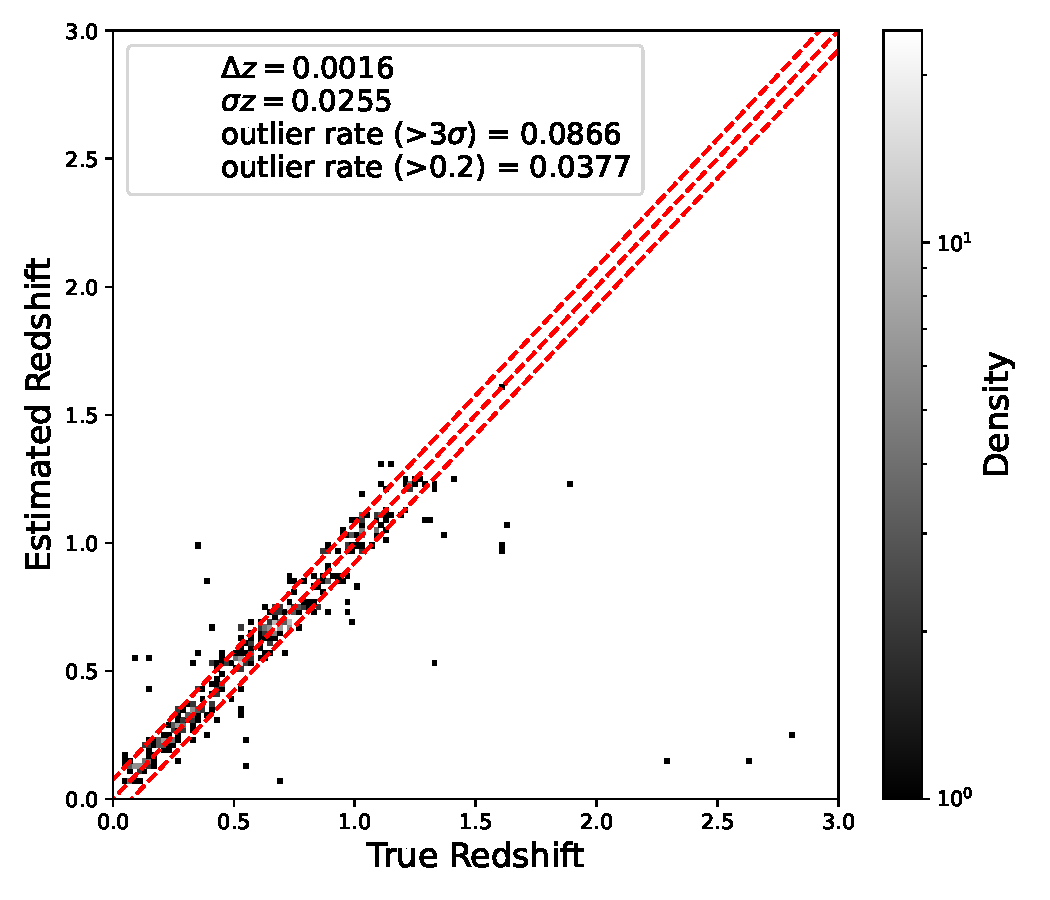
\includegraphics[width=0.45\linewidth]{figures/tpz_scatter_clean.pdf} \\
    \caption{Estimator performance for \code{TPZ} without (left) and with (right) a quality cut of $\sigma_{p(z)} < 0.15$.}
    \label{fig:scatter_quality_cut}
\end{figure*}


\subsection{Technical performance}
\label{sec:performance:technical}


\section{Limitations and caveats}
\label{sec:limitations:0}


\section{Summary and conclusion}
\label{sec:summary:0}


\section{Data Products}
\label{sec:products:0}


\subsection{Configuration files}
\label{sec:products:configuration}

\subsection{Ancillary input files}
\label{sec:products:ancillary}

\subsection{Estimator data models}
\label{sec:products:models}

\subsection{Redshift estimates}
\label{sec:products:estimates}

\subsubsection{Probability distributions}
\label{sec:products:estimates:pz_dist}

\subsubsection{Point estimates and summary statistics}
\label{sec:products:estimates:summary_stats}

\subsection{Performance Monitoring Plots}
\label{sec:products:monitoring}


\section{Data Distribution}
\label{sec:distribution:0}

\subsection{Distribution via the Rubin Data Butler}
\label{sec:distribution:butler}

\subsection{Distribution via the Photo-z Server}
\label{sec:distribution:linea}

\subsection{Distribution as LSDB}
\label{sec:distribution:lsdb}
